\chapter{Results}
\label{chapter:results}

\section{\mbox{B-trees} and the choice of $b$}
\label{sec:btree-b-choice}
As noted in chapter~\ref{chapter:implementation}, our implementation of
cache-aware B-trees (\texttt{dict\_btree}) was written for generic bounds
on node capacities. We experimented with several values of the B-tree parameter
$b$, which is tied to the size of a node. The results are presented in
figure~\ref{fig:btree-b-perf}.

\begin{figure}
\centering
\begin{subfigure}[t]{0.45\textwidth}
	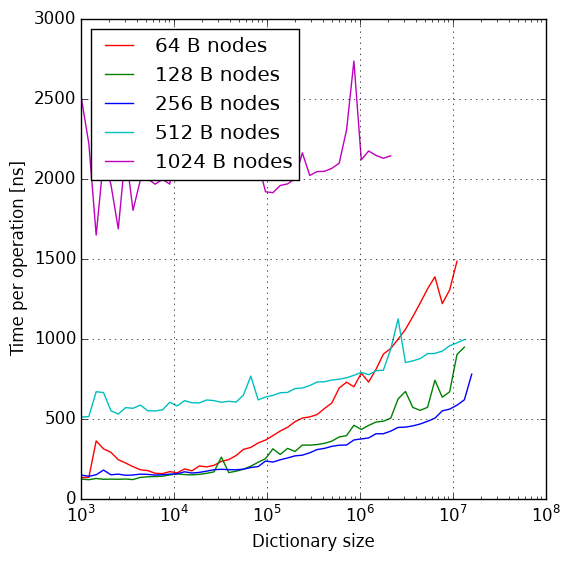
\includegraphics[width=\textwidth]{img/btree-b-find-50}
	\caption{Random \textsc{Find}s, 50\% successful (other success rates
		produce similar results)}
\end{subfigure}
~
\begin{subfigure}[t]{0.45\textwidth}
	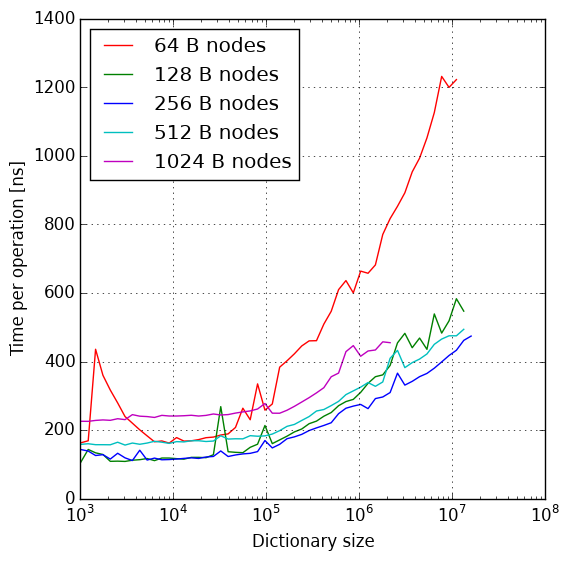
\includegraphics[width=\textwidth]{img/btree-b-insert}
	\caption{Random \textsc{Insert}s}
\end{subfigure}
\caption{The effect of different choices of $b$ on the performance of B-trees.}
\label{fig:btree-b-perf}
\end{figure}

On dictionaries larger than $10^5$ keys, a node size of $256\,\text{B}$
performed the best. However, on smaller dictionaries, it appears that
$128\,\text{B}$ might be a slightly better choice.
For all further experiments, we fixed the node size to $256\,\text{B}$
(which yields at most 15 keys per internal node).

Our code for B-trees uses linear search when looking within nodes,
as we originally did not expect the need for large nodes.
Since one node of $256\,\text{B}$ spans 4 cache lines, binary searching
within nodes might require fewer memory transfers, and hence be faster.

\section{Basic cache-aware and unaware structures}
To assess the benefits of optimizing for cache hierarchies, we compared
our optimized B-trees to simpler, cache-unaware dictiories:
red-black trees borrowed from LibUCW and a simple sorted array with binary
search and $\O(N)$ updates.
Note that in the external memory model, a binary search needs
$\Theta(\log N-\log B)$ block transfers, which is asymptotically larger than
the $\Theta(\log_B N)$ required by B-trees. Thus, theoretically lookups
on B-trees should be more efficient than binary searches on nontrivially
large dictionaries.

\begin{figure}
\begin{subfigure}[t]{\textwidth}
	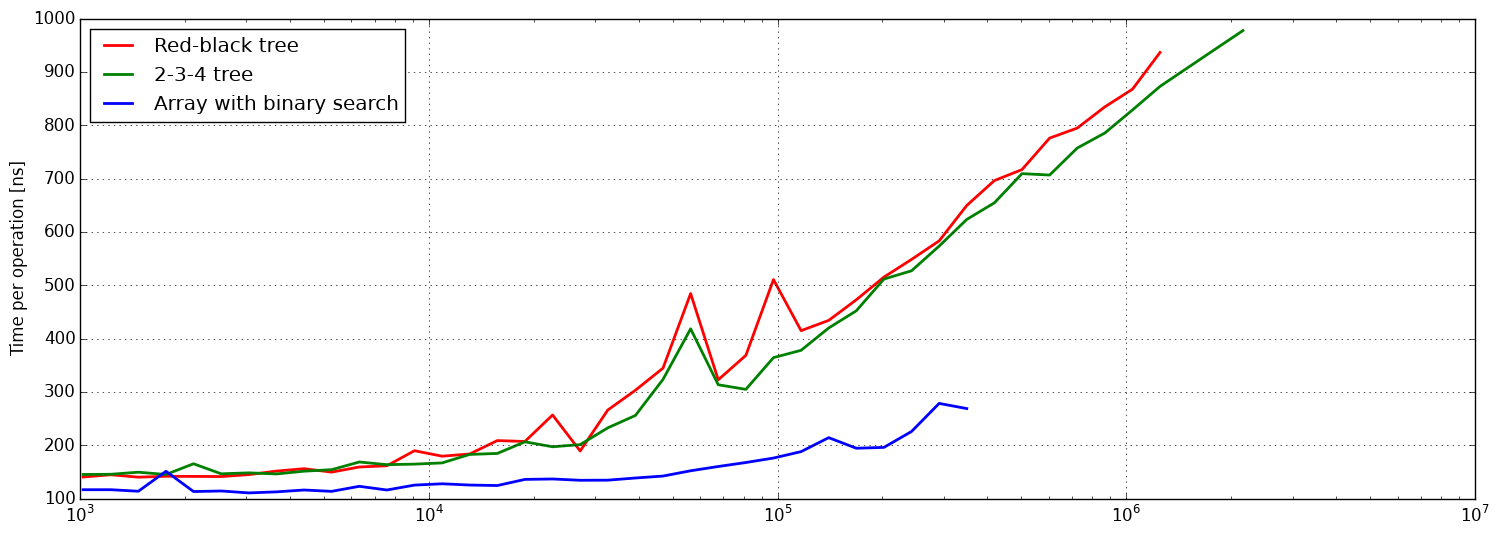
\includegraphics[width=\textwidth]{img/performance/basic-random-find-100}
	\caption{100\% success rate}
\end{subfigure}
\\
\begin{subfigure}[t]{\textwidth}
	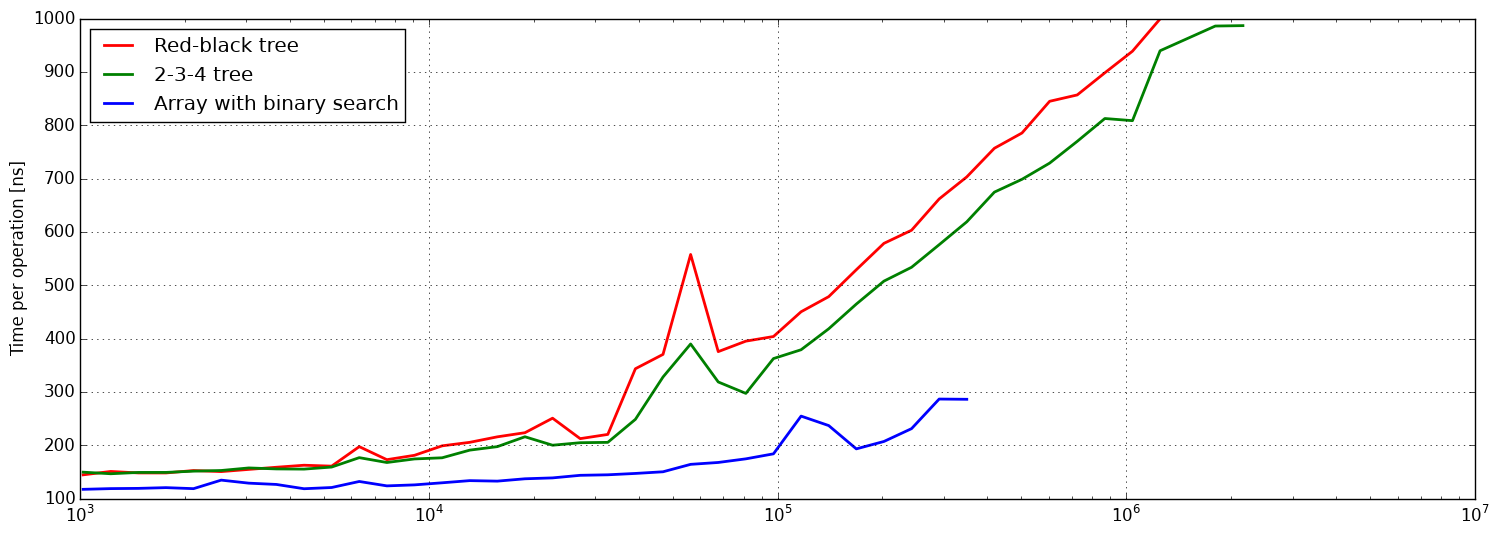
\includegraphics[width=\textwidth]{img/performance/basic-random-find-50}
	\caption{50\% success rate}
\end{subfigure}
\\
\begin{subfigure}[t]{\textwidth}
	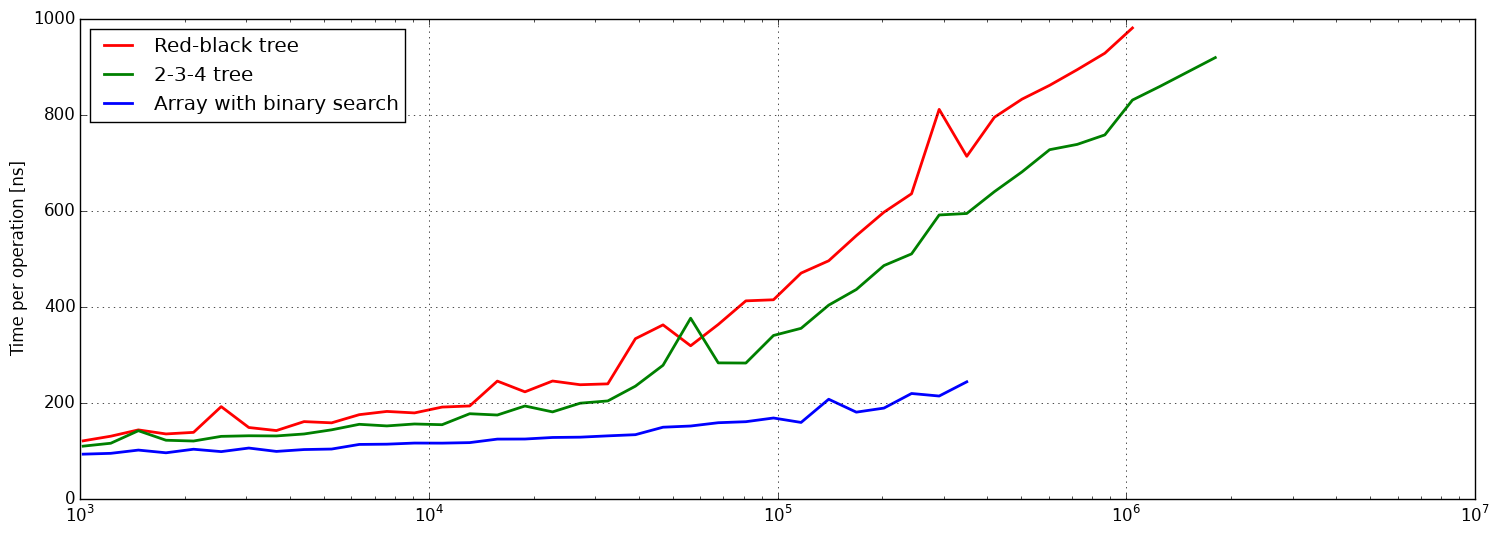
\includegraphics[width=\textwidth]{img/performance/basic-random-find-0}
	\caption{0\% success rate}
\end{subfigure}
\caption{Performance of random \textsc{Find}s in basic dictionaries.}
\label{fig:basic-finds}
\end{figure}

\begin{figure}
\centering
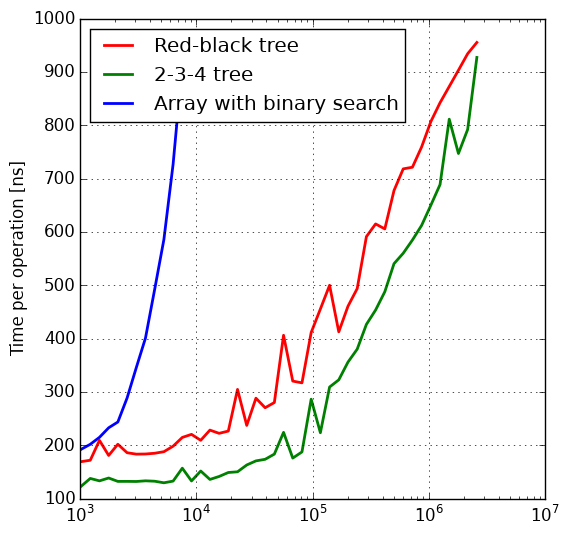
\includegraphics[width=0.5\textwidth]{img/performance/basic-random-insert}
\caption{Performance of random \textsc{Insert}s in basic dictionaries.}
\label{fig:basic-perf}
\end{figure}

Figures~\ref{fig:basic-finds}~and~\ref{fig:basic-perf} present the results.
The slow speed of operations in red-black trees (compared to binary search
and B-trees) is unsurprising.
It was, however, unexpected to find that lookups in B-trees start to overtake
binary search only on very large dictiories (with $\approx10^7$ keys).
\footnote{%
	Originally, we fixed the node size of our B-trees to $64\,\text{B}$,
	thinking it was the obviously correct choice (i.e.,\ the size of
	a~cache line). Such B-trees (or, to be more precise, 2-3-4 trees)
	were only slightly faster than red-black trees, and much slower
	than simple binary search.
	These findings prompted our suspicions and led us to trying other
	node sizes.
	As figure~\ref{fig:btree-b-perf} illustrates, our initial choice
	was actually particularly unlucky.
	The moral of this short story is that optimizing for modern machines
	is harder than it may seem.
}
Let us repeat here that B-tree \textsc{Find}s might be sped up by
replacing linear scans within B-tree nodes by binary search and repeating
the process of selecting a good value of $b$.

\section{Cache-oblivious B-tree}
\label{sec:cob-perf}
A comparison between hand-optimized B-trees and cache-oblivious B-trees is
presented in figure~\ref{fig:cob-performance}. Overall, cache-oblivious
B-trees roughly matched the performance of cache-aware B-trees.
The speed of random \textsc{Find}s was almost the same in both structures.
While cache-aware B-trees did slightly better on working set access patterns,
cache-oblivious B-trees had faster \textsc{FindNext} and \textsc{FindPrev}
operations.
\textsc{Insert} operations were about $1.5\times$ slower in cache-oblivious
B-trees.

\begin{figure}
\centering
\begin{subfigure}[t]{0.45\textwidth}
	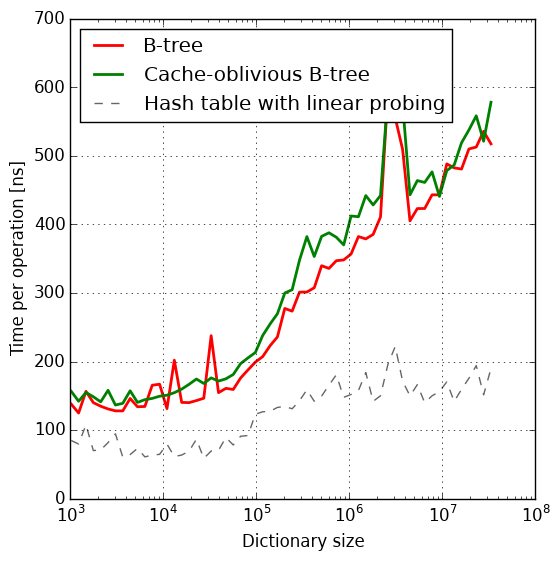
\includegraphics[width=\textwidth]{img/performance/cob-performance-1-100}
	\caption{Random \textsc{Find}s, 100\% successful (graphs for
		other success rates are similar)}
\end{subfigure}
~
\begin{subfigure}[t]{0.45\textwidth}
	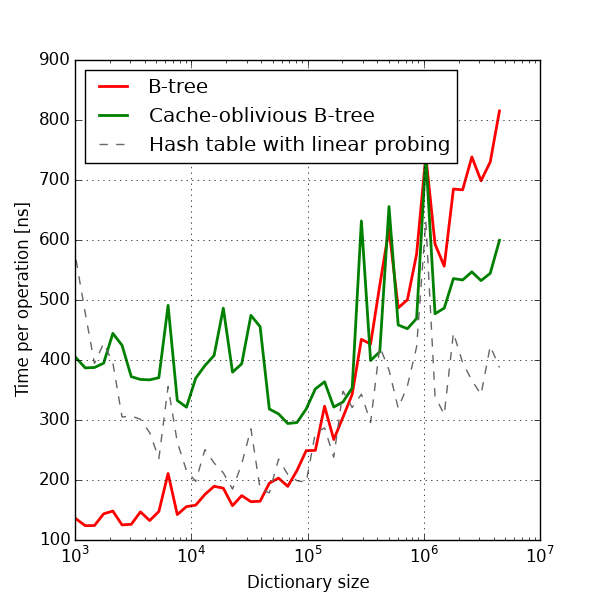
\includegraphics[width=\textwidth]{img/performance/cob-performance-2}
	\caption{Random \textsc{Insert}s}
\end{subfigure}
~
\begin{subfigure}[t]{0.45\textwidth}
	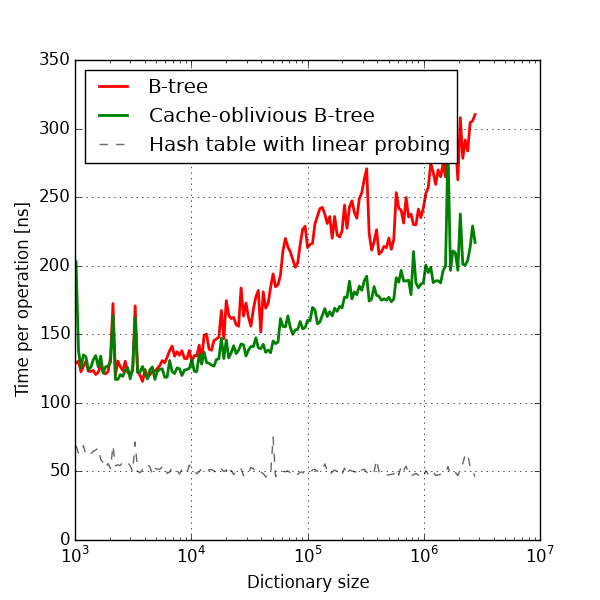
\includegraphics[width=\textwidth]{img/performance/cob-performance-3}
	\caption{Successful \textsc{Find}s, working set of 1~000 keys}
\end{subfigure}
~
\begin{subfigure}[t]{0.45\textwidth}
	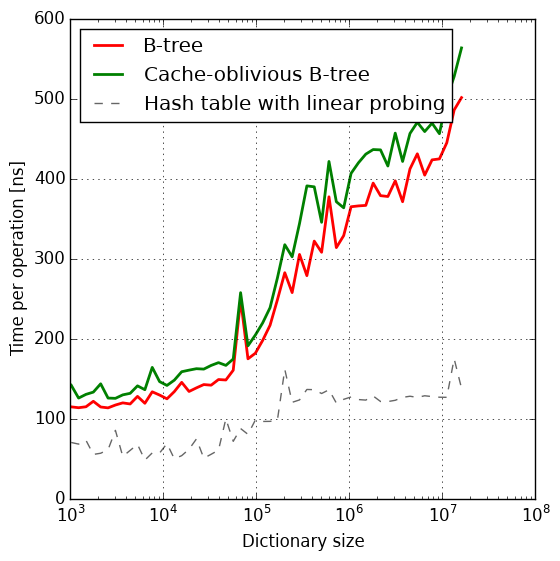
\includegraphics[width=\textwidth]{img/performance/cob-performance-4}
	\caption{Successful \textsc{Find}s, working set of 100~000 keys}
\end{subfigure}
~
\begin{subfigure}[t]{0.45\textwidth}
	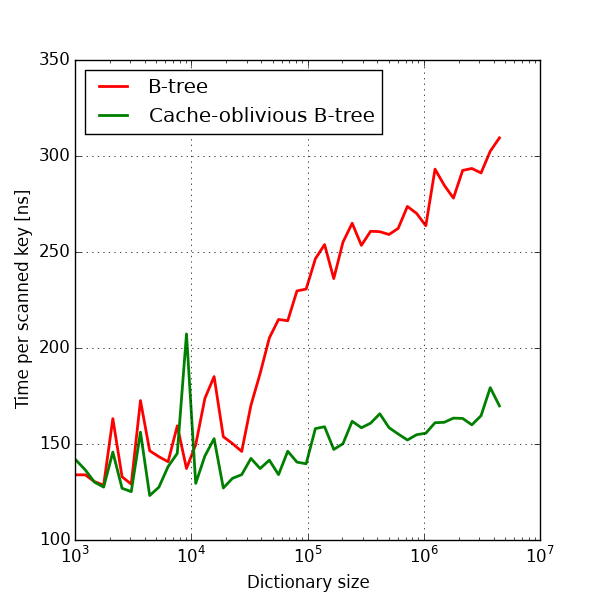
\includegraphics[width=\textwidth]{img/performance/cob-performance-5}
	\caption{Left-to-right scans over whole dictionary}
\end{subfigure}
~
\begin{subfigure}[t]{0.45\textwidth}
	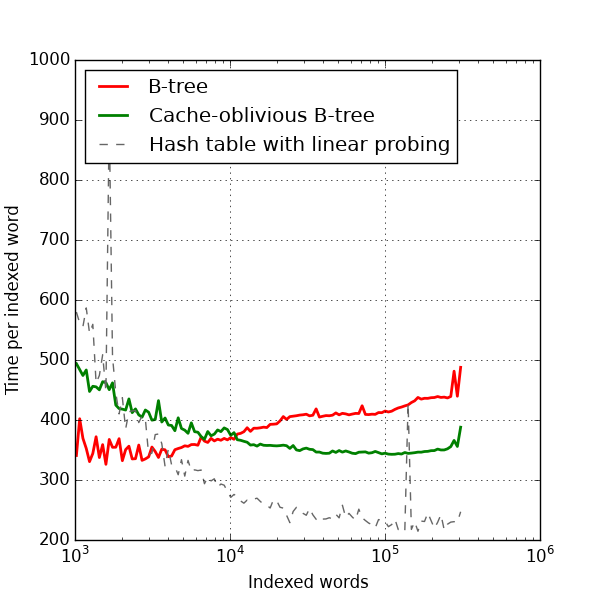
\includegraphics[width=\textwidth]{img/performance/cob-performance-6}
	\caption{Word occurrence counting}
\end{subfigure}
\caption{Benchmarks of cache-oblivious B-trees.
	Measurements of hash table with linear probing included for reference.}
\label{fig:cob-performance}
\end{figure}

\section{Self-adjusting structures}
Figures~\ref{fig:self-adj-performance-finds}~and~\ref{fig:self-adj-performance}
show a benchmark of our implementations of self-adjusting dictionaries:
splay trees, $k$-splay trees and $k$-forests.
Both figures include B-trees as a benchmark and red-black trees as a
representative of cache-unaware tree balancing schemes.
The $k$-forests are backed by our optimized B-trees, and their $k$ parameter
is picked to match our choice of $b$ (i.e.,\ $k=16$).
In $k$-splay trees, we picked $k=3$; since each $k$-splay step takes
$\Theta(k^2)$ time, we expect that higher values $k$ would not give better
performance.  % TODO: Experiment.

Splay trees are the canonical self-adjusting structure we would like to
outperfrom. As expected, splay trees are much slower than optimized B-trees.
Red-black trees are also faster than splay trees, through less dramatically
than B-trees. Interestingly, splay trees were slower in every experiment,
including experiments specifically aimed at exploiting the working set
property.

\begin{figure}
\begin{subfigure}[t]{\textwidth}
	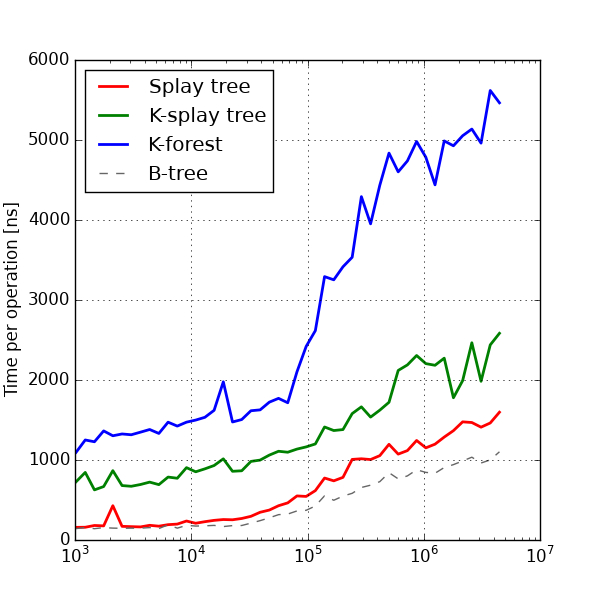
\includegraphics[width=\textwidth]{img/performance/self-adj-random-find-100}
	\caption{100\% success rate}
\end{subfigure}
\\
\begin{subfigure}[t]{\textwidth}
	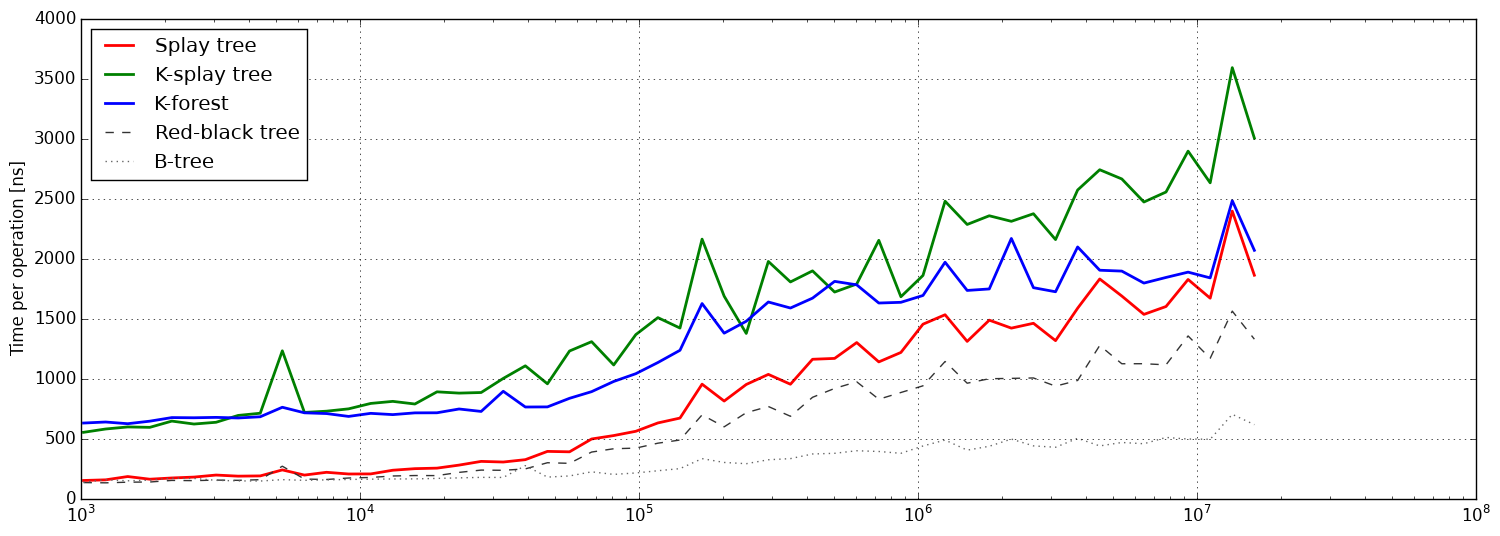
\includegraphics[width=\textwidth]{img/performance/self-adj-random-find-50}
	\caption{50\% success rate}
\end{subfigure}
\\
\begin{subfigure}[t]{\textwidth}
	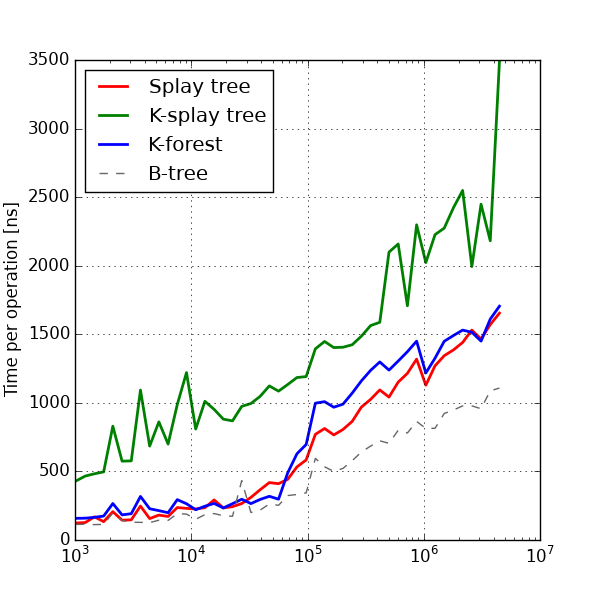
\includegraphics[width=\textwidth]{img/performance/self-adj-random-find-0}
	\caption{0\% success rate}
\end{subfigure}
\caption{Performance of random \textsc{Find}s in self-adjusting structures}
\label{fig:self-adj-performance-finds}
\end{figure}

\begin{figure}
\begin{subfigure}[t]{0.31\textwidth}
	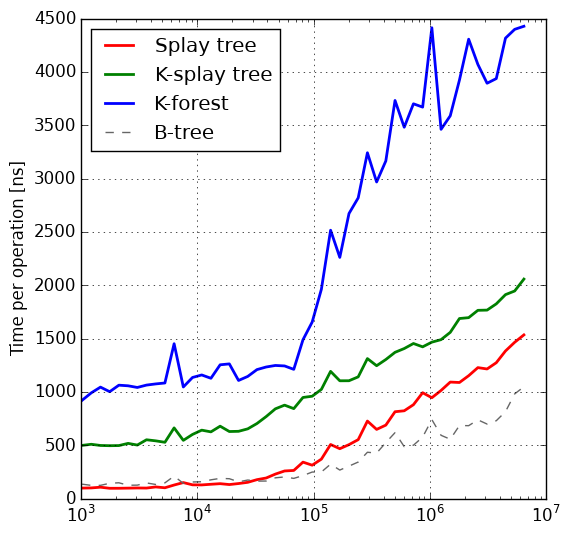
\includegraphics[width=\textwidth]{img/performance/self-adj-random-insert}
	\caption{Random \textsc{Insert}s}
\end{subfigure}
~
\begin{subfigure}[t]{0.31\textwidth}
	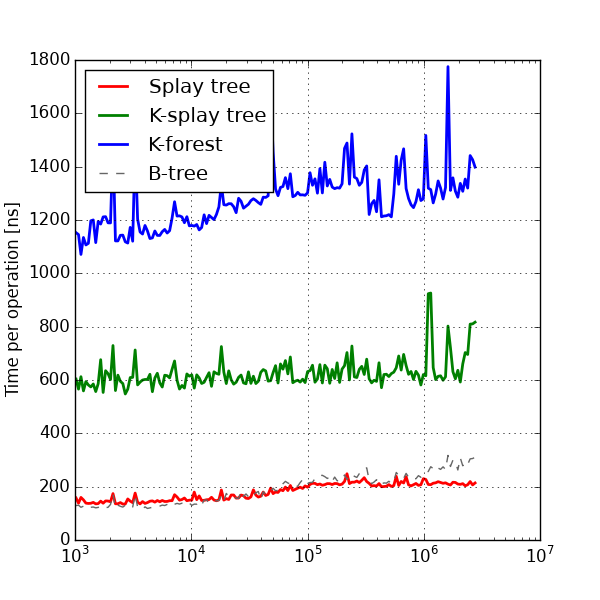
\includegraphics[width=\textwidth]{img/performance/self-adj-ws-1k}
	\caption{Successful \textsc{Find}s, working set of 1~000 keys}
	\label{fig:sub:self-adj-ws-1k}
\end{subfigure}
~
\begin{subfigure}[t]{0.31\textwidth}
	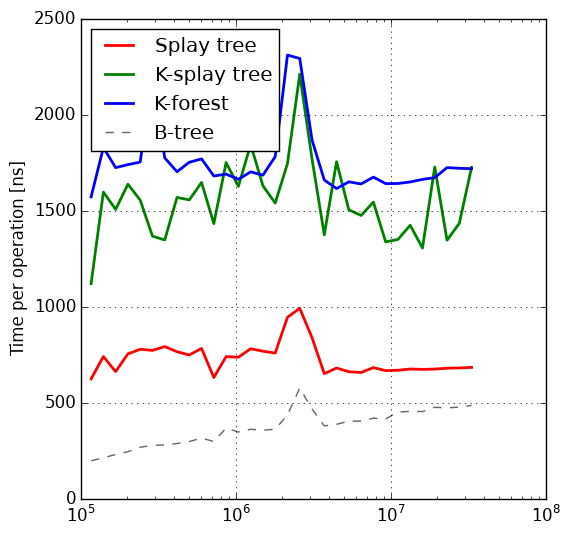
\includegraphics[width=\textwidth]{img/performance/self-adj-ws-100k}
	\caption{Successful \textsc{Find}s, working set of 100~000 keys}
	\label{fig:sub:self-adj-ws-100k}
\end{subfigure}
% TODO: word occurrence counting
\caption{Benchmarks of self-adjusting structures.}
\label{fig:self-adj-performance}
\end{figure}

Regarding the speed of random \textsc{Find}s, neither $k$-forests nor $k$-splay
trees managed to outperform splay trees. Interestingly, unsuccessful
\textsc{Find}s in $k$-forests are much faster than successful ones. This
suggests that reading from all trees of a $k$-forest is much cheaper than
promoting within a limited number of trees. It might be possible to improve
$k$-forests by switching to a backing structure with simpler demotions and
promotions.

Profiling our performance tests running on $k$-splay trees showed that about
21\% of time is spent in \texttt{ksplay\_walk\_to}, which finds the correct
leaf for a key and puts the path to the leaf into a buffer. About 37\% of the
time is taken by \texttt{ksplay\_step}, which performs a splaying step, along
with helper functions it calls (\texttt{flatten\_explore},
\texttt{compose\_twolevel}).

One suboptimal property of our implementation is that it dynamically
allocates the $k$-splayed path on every $k$-splay. Memory allocation alone
accounts for about 20\% of CPU time.
We experimented with replacing memory allocation with a static array.
This change brought the performance of $k$-splay trees somewhat closer to
splay trees, but splay trees still won in every test
(see figure~\ref{fig:ksplay-noalloc}).

\begin{figure}
\begin{subfigure}[t]{0.48\textwidth}
	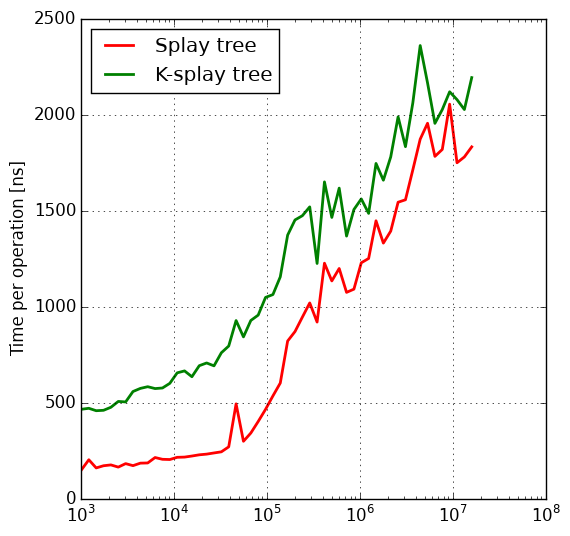
\includegraphics[width=\textwidth]{img/ksplay-noalloc-find-50}
	\caption{Random \textsc{Find}s, 50\% success rate}
\end{subfigure}
~
\begin{subfigure}[t]{0.48\textwidth}
	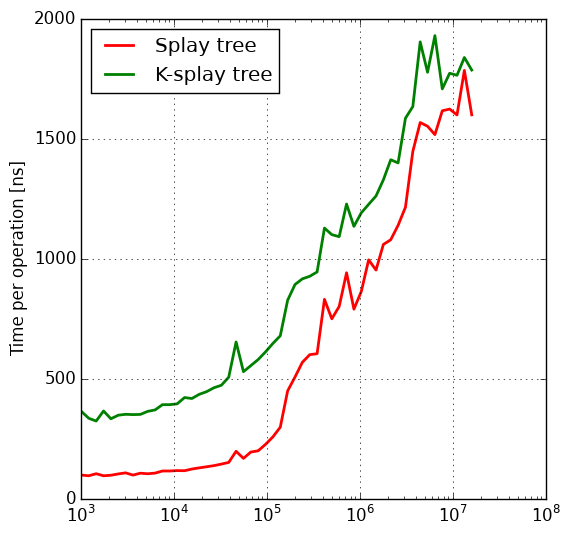
\includegraphics[width=\textwidth]{img/ksplay-noalloc-insert}
	\caption{Random \textsc{Insert}s}
\end{subfigure}
\caption{The performance of $k$-splay trees with removed temporary heap
	allocation, compared to splay trees}
\label{fig:ksplay-noalloc}
\end{figure}

As suggested in \cite{ksplay-sherk}, it should be possible to remove the
need to store the splayed path by top-down \mbox{$k$-splaying}.
Unfortunately, even top-down \mbox{$k$-splaying} needs to touch
$\Theta(k^2)$ keys and pointers in every $k$-splay step, so we believe top-down
\mbox{$k$-splaying} would not significantly reduce the high cost of
\texttt{ksplay\_step}.

Our measurements on small working sets
(figure~\ref{fig:self-adj-performance}\subref{fig:sub:self-adj-ws-1k},
\subref{fig:sub:self-adj-ws-100k}) illustrate that splay trees, $k$-forests
and $k$-splay trees have the working set property.
However, even through \mbox{B-trees} do not have the theoretical working set
property, they easily outperformed self-adjusting data structures on
benchmarks explicitly designed to benefit structures optimized for small
working sets.

\section{Hashing}
\label{sec:hashing-results}
We compared a hash table with linear probing to a cuckoo hash table.
Both hash tables used a bytewise simple tabulation hash function.
The cuckoo hash table maintained a load factor between $1/4$ and
$1/2$ and the hash table with linear probing had a load factor
between $1/4$ and $3/4$.

Since cuckoo hash tables guarantee worst-case $\O(1)$ time for lookups,
we expected both successful and unsuccessful random \textsc{Find}s to be
measurably slower with linear probing.
On random successful \textsc{Find}s (figure~\ref{fig:hashing-performance-finds}\subref{fig:sub:hashing-1-100}),
cuckoo hashing did only very slightly better than linear probing.
On unsuccessful \textsc{Find}s (figure~\ref{fig:hashing-performance-finds}\subref{fig:sub:hashing-1-0}),
the benefits of cuckoo hashing were more pronounced.
On the other hand, linear probing allows a higher load factor.
(Forcing cuckoo hashing to fill the hash tables more fully significantly
slows down \textsc{Insert}s.)

\begin{figure}
\begin{subfigure}[t]{\textwidth}
	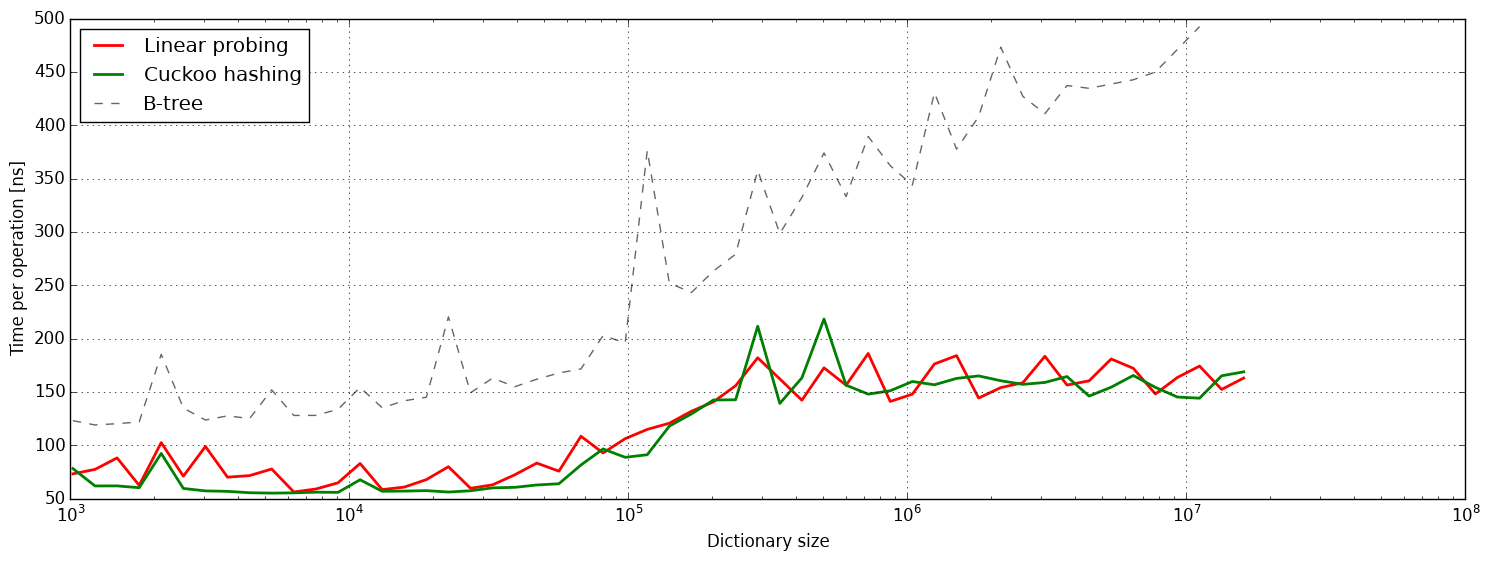
\includegraphics[width=\textwidth]{img/performance/hashing-1-100}
	\caption{100\% success rate}
	\label{fig:sub:hashing-1-100}
\end{subfigure}
\\
\begin{subfigure}[t]{\textwidth}
	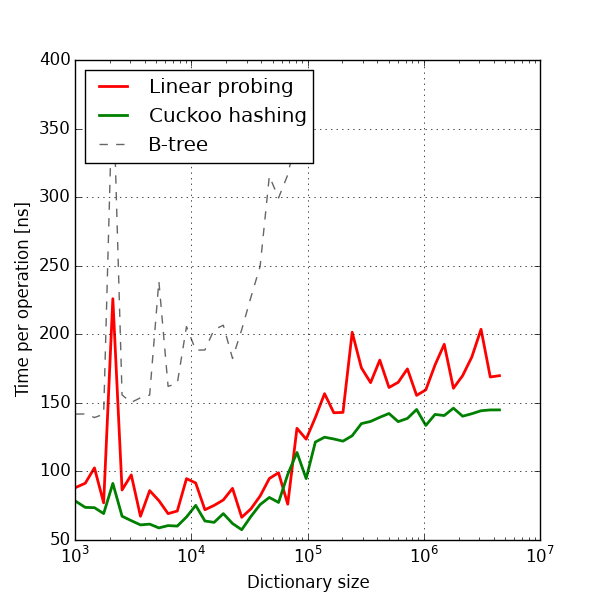
\includegraphics[width=\textwidth]{img/performance/hashing-1-50}
	\caption{50\% success rate}
\end{subfigure}
\\
\begin{subfigure}[t]{\textwidth}
	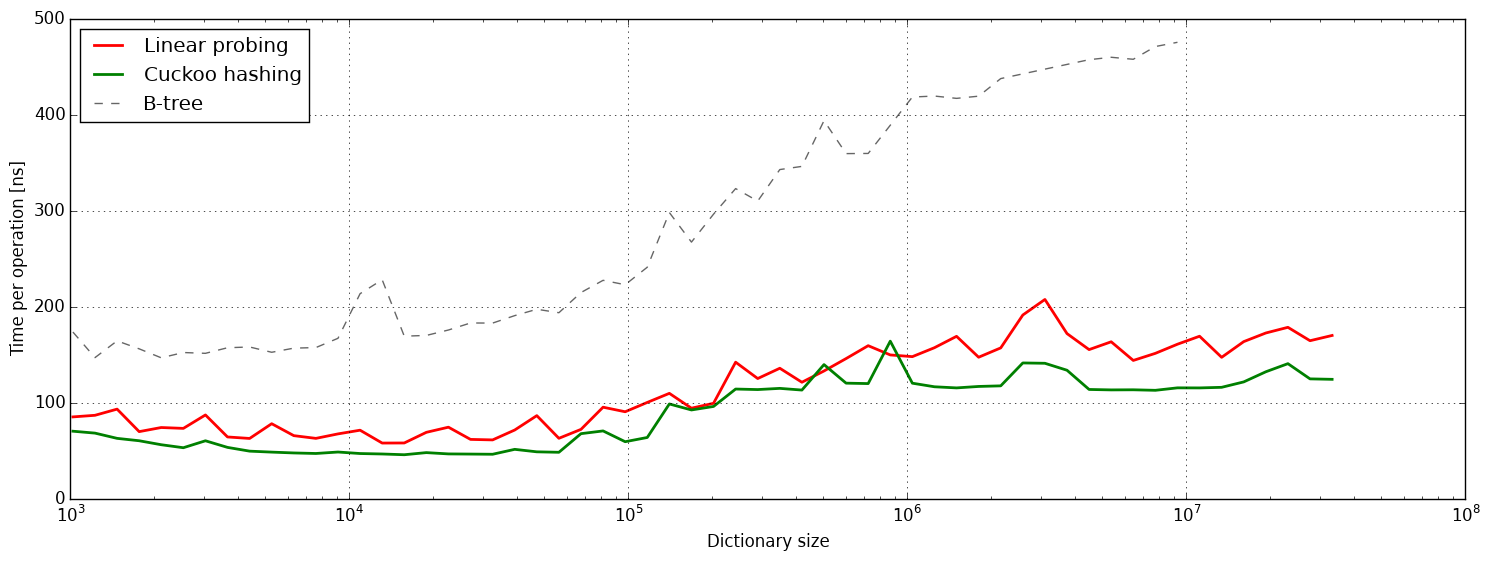
\includegraphics[width=\textwidth]{img/performance/hashing-1-0}
	\caption{0\% success rate}
	\label{fig:sub:hashing-1-0}
\end{subfigure}
\caption{Performance of random \textsc{Find}s in cuckoo hashing and linear probing}
\label{fig:hashing-performance-finds}
\end{figure}

\begin{figure}
\begin{subfigure}[t]{0.31\textwidth}
	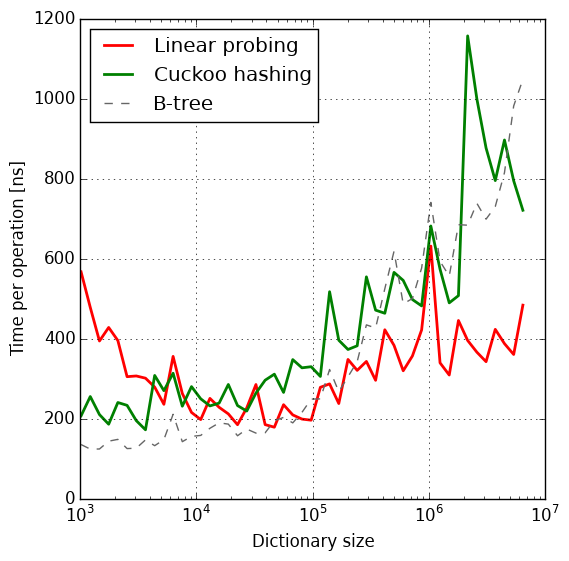
\includegraphics[width=\textwidth]{img/performance/hashing-2}
	\caption{Random \textsc{Insert}s}
\end{subfigure}
~
\begin{subfigure}[t]{0.31\textwidth}
	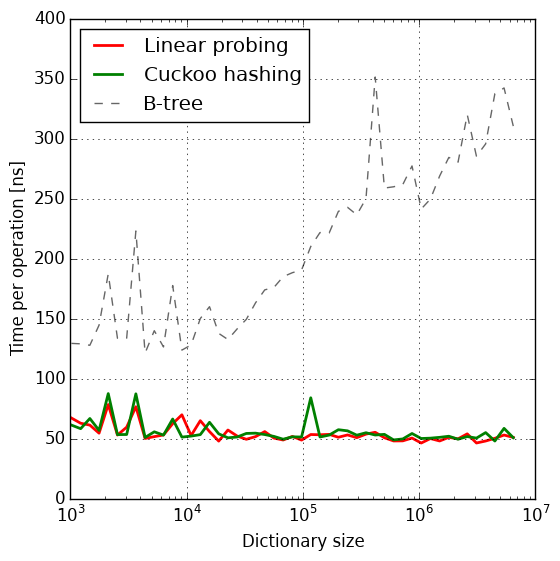
\includegraphics[width=\textwidth]{img/performance/hashing-3}
	\caption{Successful \textsc{Find}s, working set of 1~000 keys}
\end{subfigure}
~
\begin{subfigure}[t]{0.31\textwidth}
	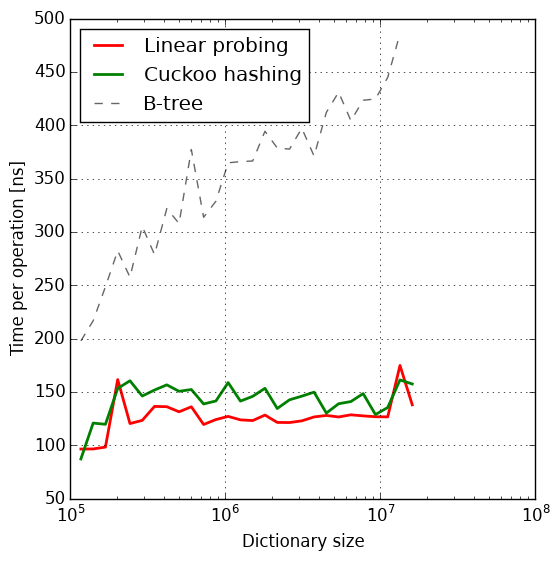
\includegraphics[width=\textwidth]{img/performance/hashing-4}
	\caption{Successful \textsc{Find}s, working set of 100~000 keys}
\end{subfigure}
\caption{Performance of cuckoo hashing and linear probing on \textsc{Insert}s
	and \textsc{Find}s in working sets}
\label{fig:hashing-performance}
\end{figure}

\textsc{Insert}s into cuckoo hash tables proved significantly slower.
One possible reason might be the limited independence guaranteed by simple
tabulation hashing.

Another interesting fact is that insertions into \mbox{B-trees} with
less than $\approx10^7$ keys were faster than inserting into hash tables
with linear probing.  % TODO: WHY?!

\section{Practical experiments}
\subsection{Mozilla Firefox}
The hash table operations collected from the Firefox session are compressed
in \texttt{data/firefox-htable.tar.gz}. We replayed the operations on all our
dictionary implementations. We normalized the measured times by the maximum
time taken for each recording to allow easier comparison of relative
performance. Table~\ref{tab:firefox-results} summarizes the results.

\begin{sidewaystable}
\centering
% TODO: Sort by best result automatically in make_table.py
\begin{tabular}{|c|r|r|r|r|r|r|r|r|r|}
	\hline
	Recording &
		Array & Red-black tree &
		B-trees & COBT &
		Splay & $k$-forest & $k$-splay &
		Linear probing & Cuckoo \\
	\hline
	\texttt{0x7f47930300e0} & 14 & 17 & 16 & 13 & 15 & 92 & 100 & 7 & \textbf{4} \\
	\hline
	\texttt{0x7fff84eb8f98} & 13 & 10 & 24 & 14 & 13 & 76 & 100 & 11 & \textbf{6} \\
	\hline
	\texttt{0x7fff1d9c7738} & 16 & 16 & 22 & 16 & 14 & 77 & 100 & 15 & \textbf{6} \\
	\hline
	\texttt{0x7fff84eb9148} & 15 & 10 & 20 & 14 & 13 & 78 & 100 & 11 & \textbf{7} \\
	\hline
	\texttt{0x7f566e3cb0e0} & 11 & 8 & 17 & 13 & 12 & 98 & 100 & 13 & \textbf{7} \\
	\hline
	\texttt{0x7f567b64a830} & 100 & 8 & 5 & 6 & \textbf{1} & 31 & 30 & 4 & 4 \\
	\hline
	\texttt{0x7f4791631c60} & 6 & 7 & 33 & 10 & \textbf{5} & 100 & 58 & 9 & 7 \\
	\hline
	\texttt{0x7f5671faab80} & 16 & 13 & 31 & 25 & \textbf{10} & 48 & 100 & 59 & 20 \\
	\hline
	\texttt{0x7f47a6e31058} & 8 & \textbf{6} & 12 & 14 & 9 & 15 & 100 & 19 & 17 \\
	\hline
	\texttt{0x7f565ca63148} & 8 & \textbf{8} & 34 & 13 & 13 & 75 & 100 & 15 & 10 \\
	\hline
	\hline
	Average & 21 & 10 & 21 & 14 & 11 & 69 & 88 & 16 & 9 \\
	\hline
\end{tabular}
\caption{Results of the Mozilla Firefox experiment. Normalized by maximum
	time (lower is better). Sorted by which implementation is fastest.
	Produced by \texttt{experiments/vcr/make\_table.py}.}
\label{tab:firefox-results}
\end{sidewaystable}

Overall, \mbox{B-trees} performed worse than our synthetic experiments would
suggest. In most cases, they were ourperformed by red-black trees, which
were slower on all synthetic experiments.
One possible explanation is the presence of \textsc{Delete}s in the recording --
we did not perform any experiment to explicitly measure their speed.

Interestingly, cache-oblivious B-trees (COBT) do not appear to have the same
problem as cache-optimized \mbox{B-trees}. This suggests that our choice
of $b$ in section~\ref{sec:btree-b-choice} may have been too biased towards
large dictionaries, which may be slowed down by a different bottleneck
than small dictionaries. Cache-oblivious B-trees avoid committing to one
$b$ via cache-obliviousness.

The winning structure in all recordings were either cuckoo hash tables,
splay trees, or red-black trees.

By inspecting the recordings, we found that splay trees are better than
cuckoo hash tables on recordings with many updates, while cuckoo tables
win when there are many more \textsc{Find}s.
We believe a data structure that would dynamically switch
its internal representation between these three data structures based
on the access pattern may be a~good compromise on small dictionaries.

Interestingly, linear probing does not behave as well on Firefox recordings
as in synthetic experiments, in which it performed as well as cuckoo hashing
in random \textsc{Find}s and slightly better on \textsc{Insert}s. One possible
reason for this is a higher incidence of failed \textsc{Insert} and
\textsc{Find} operations. As we observed in section~\ref{sec:hashing-results},
failed \textsc{Find}s are faster with cuckoo hashing, as they take only
2~memory transfers as any other \textsc{Find}, while an unsuccessful
\textsc{Find} with linear probing needs to traverse an entire chain.

\subsection{Geospatial database}
The results of the cloud database experiment are outlined in
table~\ref{tab:cloud-results}. Cache-oblivious \mbox{B-trees} slightly
outperformed standard \mbox{B-trees}. Splay trees were surprisingly fast.
One factor that might cause them to perform so well might be that stations
usually produce a~large amount of reports over their lifetime, so when we
fetch $S$~closest reports for a~point, it is likely that all such reports will
be the first $S$ reports reported by the closest station. Splay trees may thus
keep old reports near the top. In this experiment, we picked $S=1~000$. Also,
as can be seen on figure~\ref{fig:cloud-data}, the distribution of stations on
the globe is very uneven, so stations ``assigned'' to a large area can be kept
closer to the root.

Additionally, we tried two algorithms for sampling query points on the globe.
The first algorithm simply iterated through points on the latitude-longitude
grid with whole number coordinates (i.e.,\
$179.0\degree\,\text{W}\ 90.0\degree\,\text{N}$ through
$180.0\degree\,\text{E}\ 90.0\degree\,\text{S}$).
The second algorithm arbitrarily picked $64~800=180\cdot 360$ random query
points.
The algorithm can be selected by passing different values of the
\texttt{--scatter} flag to the \texttt{bin/experiments/cloud} binary
(\texttt{--scatter=GRID} for grid sampling, or \texttt{--scatter=RANDOM
--samples=64800} for random sampling).

Self-adjusting structures (splay trees and $k$-splay trees) did better
on the first one, which shows that they were probably able to take advantage
of the more predictable access pattern.

\begin{table}
\centering
\begin{tabular}{|c|S<{\,\si{\s}}|S<{\,\si{\s}}|}
% TODO: add dict_rbtree
%--close_count=1000
%--scatter=GRID
%--lat_step=100
%--lon_step=100
%--min_year=1997
%--max_year=2005 ===>
%       dict_cobt:     20 476 499 412 ns
%      dict_splay:      6 213 928 367 ns
%     dict_ksplay:     41 214 679 911 ns
%      dict_btree:     21 766 627 838 ns
%
%--samples=64800 (180*360)
%--scatter=RANDOM ===>
%       dict_cobt:     20 265 292 402 ns
%      dict_splay:      6 674 812 507 ns
%     dict_ksplay:     47 527 882 719 ns
%      dict_btree:     21 265 393 179 ns
	\hline
	Dictionary & \multicolumn{1}{c|}{Grid sampling} & \multicolumn{1}{c|}{Random sampling} \cr
	\hline
	Cache-oblivious B-tree & 20.47 & 20.27 \cr
	\hline
	Splay tree & 6.21 & 6.67 \cr
	\hline
	$k$-splay tree & 41.21 & 47.53 \cr
	\hline
	B-tree & 21.77 & 21.27 \cr
	\hline
\end{tabular}
\caption{Results of the cloud database experiment, generated
	by \texttt{bin/\allowbreak{}experiments/\allowbreak{}cloud --max\_year=2005}.
}
\label{tab:cloud-results}
\end{table}
